\section{Networking}\label{sec:sprint1-networking}
The following section will examine the different possibilities regarding transmitting player position data from the Pozyx tags to the Unity applications used to visualize the game.

\subsection{Possible networking solutions}
Unity will be used for the creation of the game aspect of this project as described in \autoref{sec:unity-intro}.
Unity includes a proprietary networking solution known as UNet \cite{unityunet}.
This solution allows developers to use a high-level API, giving access to commands that cover many common requirements for multiplayer games, without worrying about the low-level details. \\
Since the solution is developed alongside the actual game engine, it has a higher level of integration with the Unity Editor and Engine, which allows for certain components and visual aids to aid the building of the game.
As of the beginning of this project, the UNet solution has been deprecated for a while, and the Unity developers are actively working to create a new system to replace it. \\
The current UNet iteration is usable but will be removed in the future.
Other third-party solutions for Unity-based games also exist, such as Photon Engine.
Photon provides functionality for the developers to make use of to create multiplayer games in the same way as UNet, exposing higher-level functionality.
Photon supports multiple platforms outside of just Unity, with both Android and iOS support \cite{photonnet}.
\\\\
The advantage of using a library that is built for Unity such as UNet or Photon is that it is easy to set up with the Unity engine compared to a solution built from scratch.
UNet provides a higher level of abstraction with functions to control the networked state of the game, send and receive packets between server and clients and much more.\\
UNet and Photon also allow for "client-hosted" games that act like lobbies.
So any client can host a game that other clients can connect to.
This allows the clients to send and receive data between each other \cite{unityunet}.
A disadvantage of these libraries is that they are generalized and thus would not be able to achieve the same efficiency as a custom solution tailored to the specific needs of the game.
\\\\
ZeroMQ is also a possible solution.
ZeroMQ is an asynchronous packet library.
It can carry packets across various transport formats and is available in many different programming languages \cite{zeromqdoc}.
It aims to be a high-performance library to be used in distributed or concurrent applications that are reliable.
According to the getting started guide provided by ZeroMQ, certain issues tend to arise when developers attempt to create a networking solution using sockets \cite{zeromqguide}.
These are:
\begin{itemize}
    \item How to handle I/O?
    \item How are dynamic components handled? What happens if a component disappears temporarily?
    \item How are packets represented? Different sizes and different content can change representations
    \item How are packets that cannot be delivered immediately handled?
    \item Where should packet queues be stored?
    \item How are lost packets handled?
    \item What if the network transport changes, for example, TCP to UDP?
    \item How do packets get routed? Can the same packet be sent to multiple peers?
    \item How to write an API for another language?
    \item How to represent data such that it can be read between different architectures? How much of this should be the packet system's job?
    \item How do network errors get handled?
\end{itemize}
These issues are mostly applicable to general solutions that need to accommodate changing requirements or be reusable.
However, for this project, not all of these issues are relevant.
In terms of problems to overcome, this project should only be concerned with handling dynamic components, handling lost packets, routing packets and handling network errors.\\
If a player closes the game application it can lead to dynamic component issues.
A packet can be lost during the playing of the game.
Packets should be delivered to all players to ensure that they all have the same information.
Finally, a player might suddenly disconnect from the network.
\\\\
The alternative to making use of a pre-existing solution is creating a custom solution.
A custom solution entails a need to establish a familiarity with the required knowledge to construct such a solution.
A custom solution would involve sockets, which are a network API  that allows programs to communicate with each other \cite{socketnetworking}.

\subsection{Choosing a solution}
There are certain pros and cons associated with both approaches of using either a pre-existing solution or a custom solution.
\autoref{tab:networkprosandcons} shows some of the considerations made when deciding an approach for this project.
The criteria that were considered when evaluating which solution to use were:
\begin{itemize}
    \item Customizability
          \begin{itemize}
              \item How much we can customize the solution to our specific use case. If the customizability is low the project needs to be built around the networking solution, whereas if the customizability is high the networking solution can be customized to our needs.
          \end{itemize}
    \item Requirements
          \begin{itemize}
              \item How much knowledge about the subject is needed to use the solution.
          \end{itemize}
    \item Optimization
          \begin{itemize}
              \item How much optimization are we able to do ourselves if we use this solution.
          \end{itemize}
    \item Learning reward
          \begin{itemize}
              \item How much will we learn if we use this solution.
          \end{itemize}
\end{itemize}

\begin{table}[H]
    \begin{tabularx}{\textwidth}{|X|X|X|X|}
        \hline

         & \textbf{Pre-existing Unity-based}
         & \textbf{Custom}
         & \textbf{ZeroMQ}
        \\ \hline
        \textbf{Customizability}
         & Consists of a set of pre-defined functionalities
         & Can have any functionality implemented
         & Has pre-defined functionalities, but these are lower level than a pre-existing solution
        \\ \hline
        \textbf{Requirements}
         & Familiarity with the solution
         & Familiarity with the knowledge required to implement a usable solution
         & Needs familiarity with a mix of pre-existing and custom solutions
        \\ \hline
        \textbf{Optimization}
         & Lower-level details are obscured, optimized for general use
         & Lower-level details are freely available, can be optimized for a specific purpose
         & Focuses on performance, but the solution is general
        \\ \hline
        \textbf{Learning reward}
         & Most of it is already implemented, so the learning reward is low
         & Learning reward is high because we have to implement everything ourselves
         & Have to customize some of it ourselves, so we will have to get familiar with the subject
        \\ \hline
    \end{tabularx}
    \caption{A comparison of the pros and cons of the possible solutions}
    \label{tab:networkprosandcons}
\end{table}
\noindent
Based on these considerations, it was decided that a custom solution should be created to handle networking in this project.
This choice was based on two major factors: the lack of transparency in a pre-existing solution as well as the need for fast communication and the opportunity to learn more about networking at a low level. \\
For the game to be playable and enjoyable, the location data collected by the Pozyx system needs to be transmitted to all the clients as quickly as possible such that they always have an up to date view of the positions of the players.\\
To achieve this, it would be preferable to build a solution capable of performing the minimum amount of work as quickly as possible.
Pre-existing solutions cannot be guaranteed to do the minimum amount of work as lower-level details are obscured from the developers.
With a custom solution, the data sent across the network can be guaranteed to be exactly what is needed.\\
ZeroMQ was also a possible choice based on the performance needs, but its generalized approach concerning itself with reusability and issues unlikely to be a big factor in this project meant it was dismissed, in favor of a custom solution in which the problems defined in the previous section are handled.
Additionally, we have not previously worked with networking at a low level, but wanted to learn more about it, and decided that working without a framework would provide the best learning experience.

\subsection{Introduction to sockets}
In order to construct a network solution, a familiarity with the layers of a network is needed to gain an intuition of what sockets are.
A common way to describe these layers is through the \textit{open systems interconnection} (OSI) model for communication.
This model is illustrated in \autoref{fig:osi-layer}, along with approximate mappings of the technologies used for each layer.
\begin{figure}[H]
    \centering
    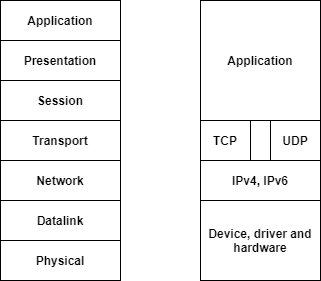
\includegraphics[width=0.6\linewidth]{networking/OSI-layer.png}
    \caption{An illustration of the OSI-layer, and the corresponding technology for each layer.}
    \label{fig:osi-layer}
\end{figure}
\noindent
As shown, the relevant layers for the purpose of creating a networking solution through sockets is the third and fourth layers, transport and network.
The network layer is handled by the IPv4 and IPv6 protocols, which will be discussed in \autoref{ipv4-ipv6}, and the transport layer is handled by either TCP or UDP, which is described in \autoref{sec:tcp-udp}.\\
The reason for the gap between TCP and UDP is to illustrate that it is possible to bypass this layer and use IPv4 or IPv6 directly \cite{socketnetworking}.
Sockets provide the interface from the upper application layers to the transport layer.
The upper layer handles details about the application, and the lower layers handle details relating to communication.
\\\\
Programs that communicate across a computer network need an agreement on how those programs will communicate.
This is known as a protocol.
Generally, before defining the design details of the protocol, a decision should be made as to which program is expected to initiate communication.
One way of defining this is through the client-server architecture illustrated in \autoref{fig:client-server}.
This split is used by most network-aware applications \cite{socketnetworking}.
The most common method of initiating communication when using the client-server architecture is to have the client initiate requests.
This tends to simplify the protocol and the programs themselves \cite{socketnetworking}.

\begin{figure}[H]
    \centering
    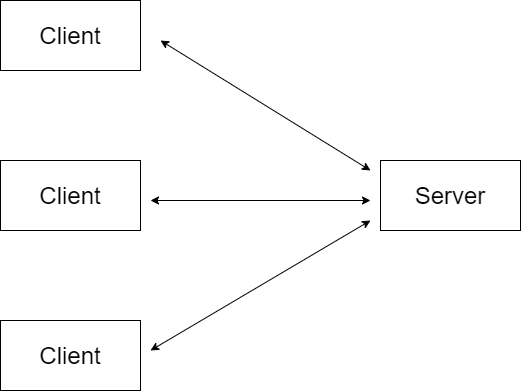
\includegraphics[width=0.6\linewidth]{networking/client_server.png}
    \caption{An illustration of the client-server architecture with multiple clients}
    \label{fig:client-server}
\end{figure}


\subsection{TCP and UDP}\label{sec:tcp-udp}
The following section introduces two different protocols for the transport layer - Transmission Control Protocol (TCP) and User Datagram Protocol (UDP).
Both of these protocols use a network-layer protocol known as IP, which can be either the protocol IPv4 or IPv6.

\subsubsection{TCP}
TCP provides connections between clients and servers.
A TCP client establishes a connection with a given server, then it receives or sends data to that server across the network and closes the connection.
TCP provides reliability by making sure that every packet that is sent is recieved by the reciever.
When TCP sends data, it requires an acknowledgment from the receiver that the data has been received.
If it does not receive such an acknowledgment, TCP automatically retransmits the data and then waits for an acknowledgment for the retransmission.
After a certain number of retransmissions, TCP gives up.\\
Based on the implementation TCP will typically attempt to send data for 4-10 minutes.
This does not guarantee that the receiver will receive the data, but the guarantee is that it will deliver the data if possible, or notify the user that the connection has been broken without an acknowledgment from the receiver.
To know how long to wait for acknowledgments, TCP contains algorithms to estimate the \textit{round-trip time} between the client and server dynamically.
It also performs these estimations continuously, as the result can be affected by variations in the network traffic.
TCP sequences data by associating bytes and sequence numbers.\\
For example, if an application writes 2048 bytes to a TCP socket, it would be sent in two segments, with the first containing data with the sequence number 1-1024, and the second containing data with the sequence number 1025-2048.
If they arrive in the wrong order, the receiving TCP reorders the segments based on the sequence numbers before passing the data to the receiving application.
If the receiver receives duplicate data this can also be detected through the sequence numbers, and the duplicate data can be deleted.\\
TCP provides flow control by telling clients how many bytes of data can be accepted at any time, known as the window.
The size of the window decreases as data is received, and increases as the receiver reads data from its buffer.

\subsubsection{UDP}
UDP is a simple transport-layer protocol \cite{socketnetworking}.
An application writes a packet to a UDP socket, which gets encapsulated in a UDP datagram, which further gets encapsulated in an IP datagram and then sent to the destination.
A datagram is a self-contained entity of data carrying information to be routed from the source to the destination nodes without reliance on earlier exchanges between the nodes and the transporting network \cite{hpbrowsernetworking}.\\
A UDP datagram is not guaranteed to reach its final destination, nor is it guaranteed that order will be preserved across the network, or that datagrams arrive only once.
This means that the UDP protocol is unreliable.
If a datagram is lost on the network and not delivered to the UDP socket, it will not be automatically retransmitted.
UDP also does not provide an acknowledgment that datagrams were received, sequence numbers to ensure data can be ordered, \textit{round-trip time} estimation or timeouts.\\\\
UDP has no notion of flow control, meaning a fast UDP sender can transmit data at a rate the receiver is unable to keep up with.
As such, it does not provide the same reliability as TCP.
If reliability is a requirement, it has to be built through features such as timeouts, retransmissions and adding acknowledgments from the receiving end.
A UDP datagram has a length, which is passed to the receiving application along with the data.
UDP is considered connectionless, as there does not need to be a long-term relationship between a UDP client and the server.\\
A UDP client can create a socket and send a datagram to a server, and then immediately send another datagram on the same socket to a different server.
A UDP server can receive several datagrams on a single UDP socket, each from different clients.


\subsubsection{Choosing between UDP or TCP}
\label{subsubsec:choosing-between-udp-or-tcp}
Windowed flow control might not be necessary for transactions where both ends agree on the maximum size of a request or a reply \cite{socketnetworking}.
For this project, the most important type of packet is the player location data.
This packet will always be formatted in the same way, and as such, a maximum size can be agreed to mean the flow control aspect of TCP is not needed.
Another aspect of TCP that is not needed for this project is the automatic retransmission of packets.
While this can provide reliability, it is of no importance for the game.\\
The players of the game are only concerned with the most recent updates of their position.
As such, if a packet were to not be received, it would not make sense to continually delay subsequent packets to attempt to retransmit a oacket containing position data that is more and more likely to be outdated.\\
For the position data to be as recent as possible, the packets should be sent as frequently as possible.
It is also not necessary to provide an acknowledgment that the packet has been received.
The receiving applications should simply update their locations to comply with the most recently received data.
The sender should not be concerned that a packet was received, it should just continue to send the next packet, which is likely to be more recent.
Duplicate packets also do not pose much of an issue.
If the applications were to receive the same location data multiple times, it would not impact the overall functionality of the program, rather just the speed at which the next updates would be received.\\
UDP has no connection setup or teardown costs.
UDP only requires two packets to exchange a request and a reply, whereas TCP requires about 10 packets \cite{socketnetworking}, if a new TCP connection is established for each exchange.
In terms of transaction time, the minimum time for a UDP request-reply is the round-trip time $+$ server processing time, and the minimum time for TCP is $2 \times$ round-trip time $+$ server processing time \cite{socketnetworking}.
\\\\
Because of the limited scope and uniformity of what is going to be transmitted via the networking solution, a lot of the features included in TCP are unnecessary.
UDP is slightly faster because of its lack of reliability and other benefits but might require some extra work to implement some of the functionality that is missing when compared to TCP if this were to become necessary.
Because of the reasons discussed, UDP seems to fit the needs of this project more than TCP and is the protocol chosen for the networking solution featured in this project.\\
An issue with the choice of UDP could present itself in that packets are not guaranteed to arrive in order.
It could pose a problem if a player in the game received a packet with recent location data, and then another packet afterward with outdated data.
This could cause the player objects in the game to be at positions in which they were in the past, but not currently in the present.

\subsection{Introduction to UDP sockets}
UDP is a connectionless, unreliable datagram protocol.
\autoref{fig:udp-client-server} shows an illustration of the client-server architecture using UDP.
The client-side creates a socket and sends a request to the server as illustrated.\\
Once the request has been sent the client transitions to a state of awaiting a reply.
Once the reply is received the client can send another request, or the socket can be closed.
The server side also creates a socket, and then binds the socket to a port.
Once bound, the server can await a request from the client.
When a request is received, the server processes it, and then sends it to the client after which it can return to awaiting requests.
\begin{figure}[H]
    \centering
    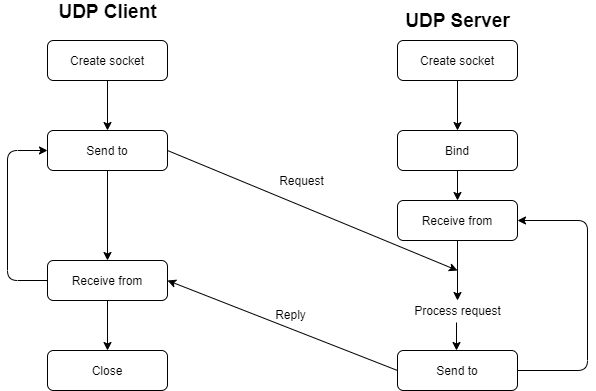
\includegraphics[width=0.6\linewidth]{networking/udp-client-server.png}
    \caption{An illustration of the client-server architecture with UDP}
    \label{fig:udp-client-server}
\end{figure}
\noindent
For the purpose of this project, it might not be optimal to have client request the server.
The server does not need information from the client or acknowledgment, meaning the clients do not have to send packets.
As such, it might be better to use a publisher-subscriber approach.\\
The server would then act as a publisher, constantly sending packets to the clients that would be subscribed to the publisher.
An illustration of this concept using UDP can be seen in \autoref{fig:udp-pub-sub}.
\begin{figure}[H]
    \centering
    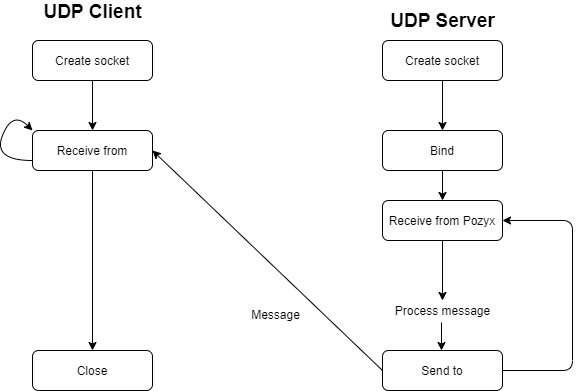
\includegraphics[width=0.6\linewidth]{networking/pubsubudp.png}
    \caption{An illustration of a publisher-subscriber architecture with UDP}
    \label{fig:udp-pub-sub}
\end{figure}
\noindent
Possible issues with using this architecture is that there would need to be a way to ensure all clients receive a sufficient amount of packets, and that the receivers are not overloaded with packets.

\subsubsection{Transmission in UDP}\label{sec:sprint1-udptransmission}
When working with UDP, there are three types of possible transmissions: Unicast, multicast or broadcast.
Unicast is a one-to-one communication with a single source sending information to a single receiver, while a broadcast transmits the information to all nodes on a network.\\
The benefit of unicast is that it has been in use for a long time and utilizes well-established protocols, it is known from applications like HTTP, FTP, and Telnet \cite{finjan}.
For this project, however, the major drawback of unicast is that to transmit the packet to multiple nodes, it has to send multiple unicasts packets addressed to each receiver, which also requires us to know the exact IP address of each destination device.\\
Looking at broadcast, we can instead transmit the information to all nodes on a network, which ensures that all nodes on the network receive the packet.
This could be useful if we only had the players of the game on our network, but since they might be connected to a larger network with a large number of clients, this could lead to the data being sent to clients that are not a part of the ongoing game session.\\
Luckily, we have multicast in the middle of the two extremes, where you do not send from one client to another or one client to all others.\\
Instead, the data is sent to as many destinations as express an interest in receiving it \cite{finjan}.
This one-to-many approach seems suitable for this project since it would intuitively lead to better bandwidth utilization and does not require the receivers' addresses to be known.

\subsection{IPv4 and IPv6}\label{ipv4-ipv6}
Both IPv4 and IPv6 provide packet delivery service for TCP and UDP.
The major difference in IPv4 and IPv6 is the addresses they use.
IPv4 uses 32-bit addresses, whereas IPv6, being a newer version, uses larger addresses of 128 bits \cite{socketnetworking}.
IPv4 addresses are usually written as four decimal numbers separated by ".".
This is known as \textit{dotted-decimal notation}.\\
Each decimal number represents one of the four bytes of the 32-bit address.
The first of the four numbers represent the address type.
IPv6 addresses are usually written as eight 16-bit hexadecimal numbers \cite{socketnetworking}.
The higher-order bits of the 128-address imply the type.
For this project, this should not have a significant impact, and either can be used.


\subsection{Format of data}\label{subsec:data-format}
As it is necessary to send data over the network, the format of the data must be decided upon.
The network format for player position and goal position is \texttt{0xyyyyxxxxiisstt}, where \texttt{t} is the type, \texttt{s} is the timestamp, \texttt{i} is the ID, \texttt{xxxx} is the \texttt{x} position and \texttt{yyyy} is the \texttt{y} position.
The format can be seen for the player positions on \autoref{Tab:player-format}.
The format is little-endian, as the most significant byte is the one related to type, which is placed at the end.
The abstract syntax for these packets is:
\begin{itemize}
    \item Type of the packet
    \item Timestamp
    \item ID associated with the packet
    \item X position
    \item Y Position
\end{itemize}
The format for both is identical, the only difference between them is the type of the packet and the context of the IDs.
The abstract syntax for field anchor position is nearly identical, as the same information is required, but the field anchor format does not require a timestamp.
For player position and field anchor position packets the \texttt{x} and \texttt{y} position is the location of the player or anchor.
For the goal position format the \texttt{x} and \texttt{y} position is the center of the goal, where the size of the goal is set to have a length equal to 20\% of the shortest side of the playing field.
\\\\
The IDs for each syntax represent different things.
The IDs for \autoref{Tab:player-format} are for each anchor, whereas ID for players is either the player tag or the ball tag, and the ID for the goal position packet identifies the team.
The type is represented at the right hand side of the hexadecimal so that it is faster to decode and to switch on which type it is.
After the type the timestamp is placed, which is used to detect outdated data as a sequence number.
The timestamp is an integer value ranging between 0 and 255 such that when it hits 255 it resets to 0 to be able to continuously send timestamps, regardless of game length.
The downside to this approach is since UDP does not guarantee delivery of packets, it may not go straight from 255 to 0 every time.
To counter this, 0 to 20 is considered as newer sequence numbers than 235 to 255 so that the system is allowed to miss up to 20 packets near the end, to ensure that it does not end up being locked until the values reach the high range again.
\\\\
It was decided to use a size of respectively 16 and 8 bits so that it is straightforward to work with in the \texttt{C\#} language, because it is the same size as some variable types in \texttt{C\#} and hereby easy to type cast.
Given the highest unsigned number that can be in two bytes is $2^{16} - 1$, the maximum value for the \texttt{x} and \texttt{y} positions is 65.535.

\begin{table}[h!]
    \centering
    \begin{tabular}{|l|l|l|l|l|}
        \hline
        \begin{tabular}[c]{@{}l@{}}POSY (y)\\ (0-65.535)\end{tabular} & \begin{tabular}[c]{@{}l@{}}POSX (x)\\ (0-65.535)\end{tabular} & \begin{tabular}[c]{@{}l@{}}ID (i)\\ (0-3)\end{tabular} & \begin{tabular}[c]{@{}l@{}}TIMESTAMP (s)\\ (0-255)\end{tabular} & \begin{tabular}[c]{@{}l@{}}TYPE (t)\\ (0)\end{tabular} \\ \hline
        16 bits                        & 16 bits                        & 8 bits                         & 8 bits                         & 8 bits                         \\ \hline
    \end{tabular}
    \caption{Format for player positions}
    \label{Tab:player-format}
\end{table}
\noindent
\\
The goals scored has a different format of \texttt{0x1100sstt}, where \texttt{t} is type, \texttt{s} is timestamp, \texttt{00} is the score of team 0 and \texttt{11} is the score of team 1.
This format can be seen on \autoref{Tab:goals-scored-format}.

\begin{table}[h!]
    \centering
    \begin{tabular}{|l|l|l|l|}
        \hline
        \begin{tabular}[c]{@{}l@{}}TEAM1SCORE (1)\\ (0-100)\end{tabular} & \begin{tabular}[c]{@{}l@{}}TEAM0SCORE (0)\\ (0-100)\end{tabular} & \begin{tabular}[c]{@{}l@{}}TIMESTAMP (s)\\ (0-255)\end{tabular} & \begin{tabular}[c]{@{}l@{}}TYPE (t)\\ (3)\end{tabular} \\ \hline
        8 bits                         & 8 bits                         & 8 bits                         & 8 bits                         \\ \hline
    \end{tabular}
    \caption{Format for goals scored.}
    \label{Tab:goals-scored-format}
\end{table}
